\chapter{Introduction and Background}
\label{cha:intro}
This chapter briefly introduces the problem of image-to-image translation,
deep learning and Generative Adversarial Networks. General ideas of these topics
are very useful for the reader to grasp the more complicated concepts that 
the report talking about in the later chapters.

\section{Image-to-Image Translation}
\subsection{Definition}
Many challenges in computer vision and machine learning can be regarded as “translating” an 
input image into a corresponding output image. As we all know that a concept may be expressed in either 
English or Chinese, a scene can be represented as various forms including RGB images, gradient fields, 
edge maps, segmentation maps, etc. Similar to machine translation of languages, we cite the definition
of image translation from Isola et al.: “tasks of automatically translating
one possible representation of a scene into another”\cite{pix2pix2016}. Researchers have solved some kinds of image 
translation using independent, specific-purpose machinery(e.g. style transfer\cite{gatys2015neural}),
even if the settings of these problems are the same: predict pixels from pixels.
The models this report discuss (originated from \cite{pix2pix2016})
make using one common framework for all these problems possible.
In this project, we will focus on translating 
semantic segmentation maps into photorealistic images but you can apply these approaches on
other types of image translation problems.

\subsection{Segmentation Maps}
In computer vision, image segmentation is often needed in order to switch to 
different representations of an image especially to those representations that 
are more meaningful and simpler for analysis\cite{wikipedia},
and a lot of deep learning algorithms have been invented to do semantic labeling. Therefore,
the data this project needs is easy to acquire.

Segmentation maps are also known as semantic label maps, which is a set of segments 
that collectively cover the entire image\cite{wikipedia}. Each region contains similar pixels 
in terms of the semantic of the image and each region is assigned with a different 
color and a semantic label.

The following figure \ref{fig:segmentation-map-example} is an example segmentation map image, where each color represent one type of object:
\begin{figure}[H]
    \begin{center}
    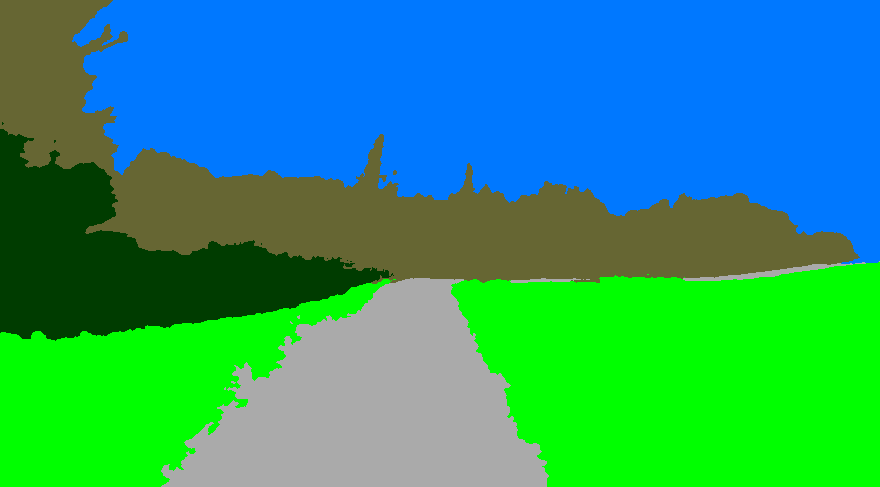
\includegraphics[width=8cm]{figures/seg-map-eg}
    \end{center}
    \caption{A Segmentation Map}
    \label{fig:segmentation-map-example}
\end{figure}

\subsection{Applications}
The translation of photorealistic images from sketches will be very useful once this technology
is mature enough for commercial uses. Designers could get a fast preview of 
their work not by imagination, but with vivid photorealistic images. For example, 
game designers can preview the scene, items, or characters they design vividly by drawing 
just sets of color blocks or edges. Besides, this technology provides opportunities for 
people who are not good at art to create their own masterpieces.


\section{Deep Learning}
\nocite{articleDL}
\nocite{Goodfellow-et-al-2016}
Deep learning is a member of the machine learning algorithms family, based on
artificial neural networks and representation learning\cite{wikipedia}(i.e. automatically discover 
representations needed for feature detection or classification from raw data). 
Learning can be supervised, semi-supervised, or unsupervised. Deep learning approaches have widely
been applied to fields including computer vision(CV), natural language processing(NLP), 
reinforcement learning(RL), text filtering, machine translation, image synthesis, drug design, etc., 
where they perform comparably to and in some cases better than human experts.  

\subsection{Neural Networks}
Artificial neural networks(ANN) are computing systems vaguely inspired by 
the biological neural networks that constitute animal brains\cite{wikipedia}. Neural networks used in deep learning 
can be regarded as a parametric approximation function that can map the input A into the output
B with parameters $\omega$ i.e. $f_{\boldsymbol{\omega}}: A \rightarrow B$. The mapping 
function can gradually get optimized by updating its parameters through raw data and 
back propagation algorithms. 

The multi-layer architecture of neural networks can achieve complex mappings by composing 
multiple but simple non-linear functions together.
In neural network implementations, the input “signal” will pass into each neuron(or node) through
connection edges, the output of each neuron is computed by some non-linear function of 
the sum of its inputs, typically, neurons are aggregated into layers and the “signals”
travel from the first input layer to the last output layer to produce the final results.
\begin{figure}[H]
    \begin{center}
    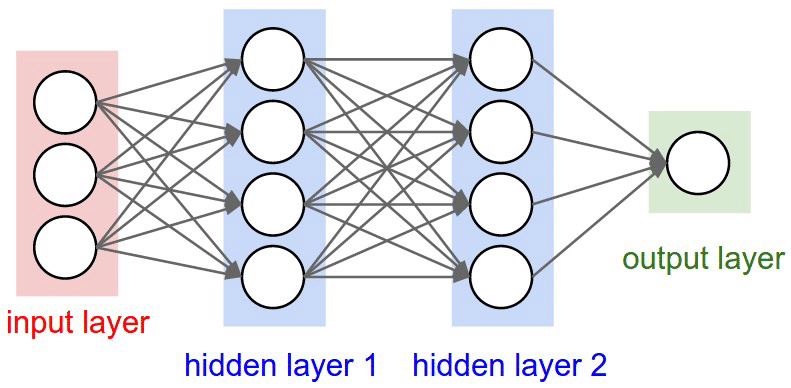
\includegraphics[width=8cm]{figures/nn-structure}
    \end{center}
    \caption{Neural Network Structure}
    \label{fig:neural-network-structure}
\end{figure}

\subsection{Activation Functions}
The activation function of a node(i.e. neuron) in neural networks determines the output of that node 
given an input or set of inputs. Note that only non-linear activation functions allow such networks 
to compute complex mappings, if we do not use activation function or use linear activation function,
no matter how many layers we have, we can only result in getting linear mapping functions.

The activation functions this project uses are the following(explanations referenced from \cite{cs231n}):
\begin{itemize}
    \item Rectified Linear Unit(ReLU)
    
    The Rectified Linear Unit is one of the simplest and most commonly used activation functions 
    in the last few years, it computes the function: $f(x)=\max(0,x)$. 
    This activation function is just threshold at zero, which is much simpler than tanh or sigmoid, 
    and it was found to greatly accelerate the convergence of gradient descent compared to other 
    activation functions including tanh or sigmoid. However, it does has a disadvantage of being fragile
    during training, i.e. the ReLU units can irreversibly die and forever be zero during training since 
    they can get knocked off the data manifold. 
    \begin{figure}[H]
        \begin{center}
        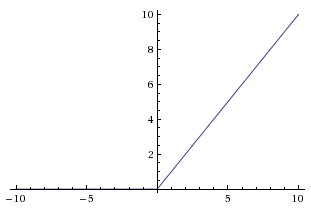
\includegraphics[width=5cm]{figures/relu}
        \end{center}
        \caption{Rectified Linear Unit(ReLU) Activation Function}
        \label{fig:ReLU}
    \end{figure}
    \item Leaky Rectified Linear Unit(Leaky ReLU)
    
    Leaky ReLUs are one type of approach trying to fix the "dying ReLU" problem. Instead of just threshold 
    at zero, it computes: $f(x)=1(x<0)(\alpha x)+1(x>=0)(x)$, where $\alpha$ is a small constant. Some report 
    leaky ReLUs are effective but the reuslts are necessarily consistent.
    \begin{figure}[H]
        \begin{center}
        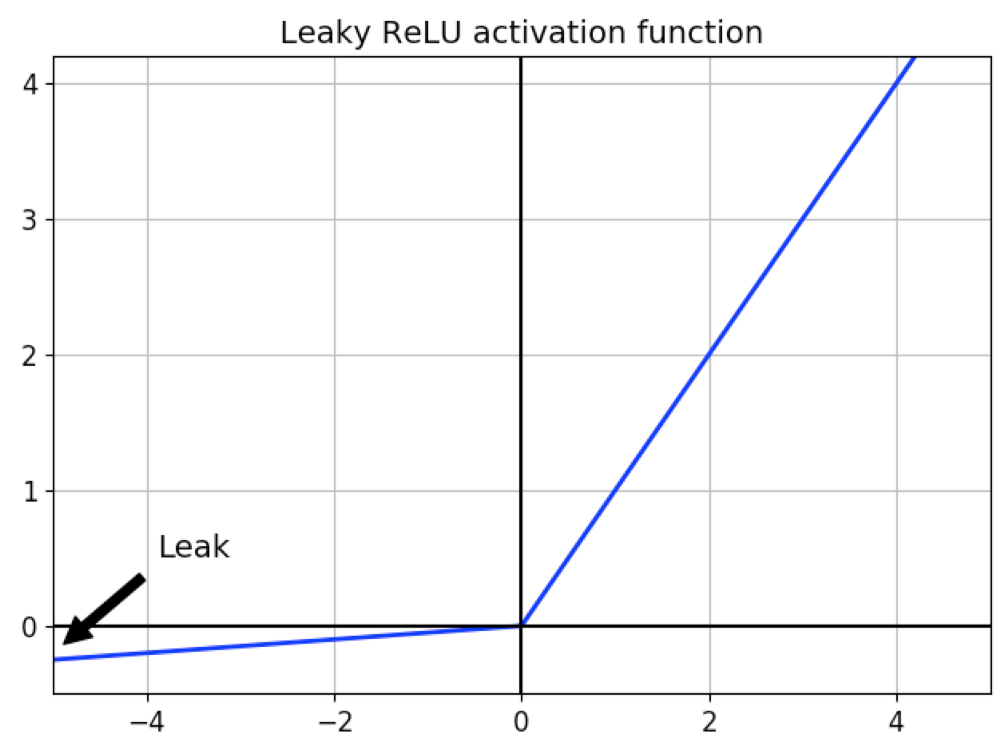
\includegraphics[width=5cm]{figures/leakyrelu}
        \end{center}
        \caption{Leaky ReLU Activation Function}
        \label{fig:Leaky ReLU}
    \end{figure}
    \item Hyperbolic Tangent(tanh)
    
    The tanh activation function squashes a real-valued number to the range of [-1, 1], this activation
    saturates but is zero-centered so that it can be regarded as a scaled and more desirable sigmoid 
    activation function in practice.
    \begin{figure}[H]
        \begin{center}
        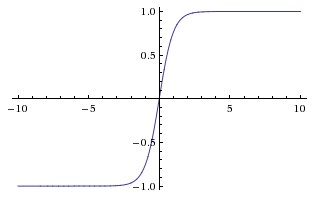
\includegraphics[width=5cm]{figures/tanh}
        \end{center}
        \caption{Hyperbolic Tangent Activation Function}
        \label{fig:tanh}
    \end{figure}
    
\end{itemize}

\subsection{Backpropagation}
Backpropagation(BP) is a widely used algorithm for neural networks training and
supervised learning. While training a neural network, there will be a loss function
$L$ describing how well the current approximation $f_{\boldsymbol{\omega}}$ approximates
the correct mapping function by calculate the differences between the output from the 
neural network and the ground-truth from a training dataset. Then the backpropagation algorithm 
will try to approximate the correct mapping function by continuing minimizing the loss function, 
this can be done by computing the gradients of the loss function with respect to 
each weight from each pair of input-output data by the chain rule, 
computing the gradient one layer at a time, iterating backward from the last layer to 
the first(in order to avoid redundant computation) and update every parameter 
${\boldsymbol{\omega}_{i}}$ using 
$\boldsymbol{\omega}_{i} \leftarrow \boldsymbol{\omega}_{i}-\alpha \frac{\partial L}{\partial \boldsymbol{\omega}_{i}}$
where $\alpha(>0)$ is the learning rate and $\frac{\partial L}{\partial \boldsymbol{\omega}_{i}}$ is the partial
derivative(i.e. gradient). Theoretically, the gradient has the direction away from the minimal point, 
so each time of these updates will make the neural network 
approximate better by taking a little step in the opposite direction of the gradient, this idea 
of minimizing the loss function is called gradient descent.

\subsection{Convolutional Neural Network}
Convolutional Neural Network(CNN) is a popular type of deep neural networks which commonly applied to 
the computer-vision-related tasks. 
A typical Convolution block consists of a convolution layer, a pooling layer and a 
fully-connected layer(exactly the same as regular neural network). A simple pipeline could be:
[INPUT-CONV2D-ACTIVATION-POOLING-FC], In more detail(explanations cited from \cite{cs231n}):
\begin{itemize}
    \item INPUT [width, height, channels] will hold the raw pixel values of an input image, for example, for MNIST
    would be [28, 28, 1], i.e. 28x28 resolution images with only one channel for the black and white colors.
    \item CONV2D is the key of the convolutional neural network, the convolution layer 
    will compute the output of neurons that are connected to local regions in the input, each 
    computing a dot product between their weights and a small region they are connected to the input volume.
    The shape of the output tensor will be [width, height, filters], where the number of filters is a hyperparameter for our 
    CNN layer. The convolution layer can extract related feature maps from the original images(e.g. edges, corners, etc.)
    with appropriately optimized parameters, which is very useful for further analysis 
    such as classification or generation. 
    \item ACTIVATION is easy to understand, we can simply use RELU(or leaky RELU, tanh), this will not change 
    the shape of the output tensor.
    \item POOLING: in most cases, we will use max pooling, which is typically a downsampling operation along the 
    spatial dimensions(width, height), and change the output tensor shape to [width/n, height/n, filters].
    \item FC, fully-connected layer, each neuron in this kind of layer will be connected to 
    all the numbers in the previous volume.
    For instance, in a classification task, a fully-connected layer will compute the class scores 
    resulting in the shape of [1, 1, classes], where there will be a score for each class representing 
    how likely the image is that class.
\end{itemize}
In this way, CNN transforms the original image from the pixel values to encoded feature maps or classification 
class scores. Note that the reverse version of CNN called CNN transpose can decode feature maps back to images,
so in our image translation task, we will first use CNN to get the segmentation map into features maps, and then
use CNN transpose to get the feature maps to photorealistic images.
\begin{figure}[H]
    \begin{center}
    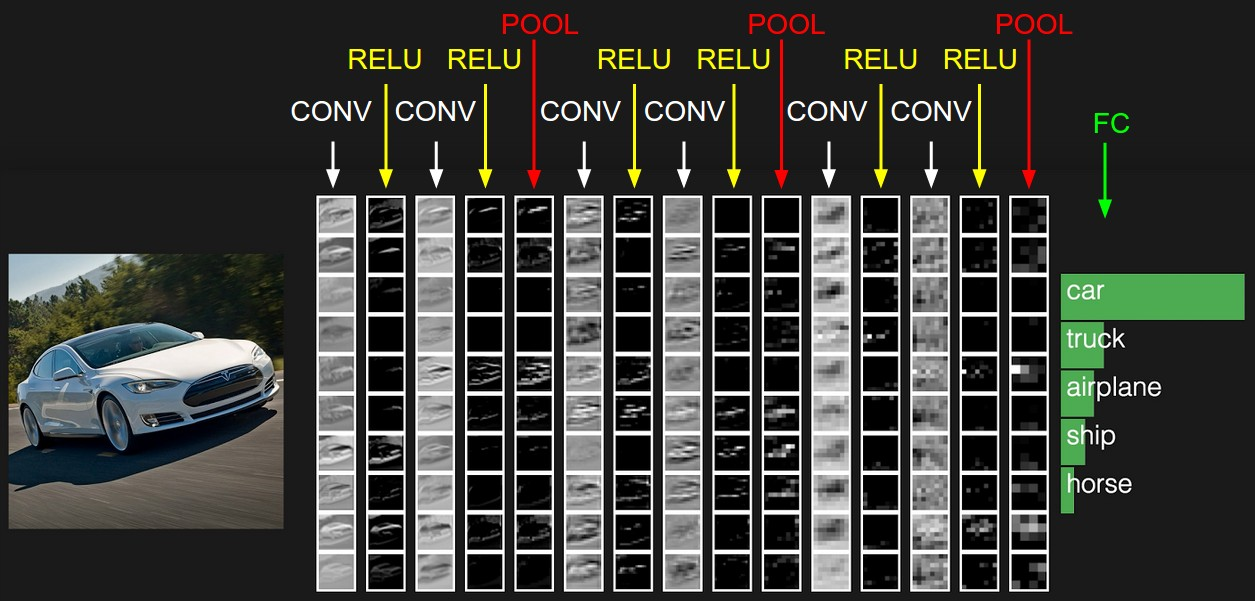
\includegraphics[width=8cm]{figures/convnet}
    \end{center}
    \caption{Example CNN Task}
    \label{fig:CNN}
\end{figure}

\subsection{Residual Blocks}
A traditional view of deep learning is that using a deeper network not necessarily results in better 
performance, in fact, simply stacking too many CNN blocks has been shown to cause a negative effect
since the gradient can easily shrink to zero. However, the ResNet with residual blocks brought by He et al. 
\cite{he2015deep} has eliminated this problem. The residual block skip connects between layers which adds
the output from previous layers $x$ to the output of stacked layers $F(x)$, in this way, even if something wrong
happens to the stacked deeper layers output(e.g. gradient vanishing), the network is still able to learn the 
identity output from the previous output. Therefore, residual blocks guarantee us to get results no worse than
a shallow network, and when this apply to CNN, a even deeper CNN can be more powerful for computer vision tasks.
\begin{figure}[H]
    \begin{center}
    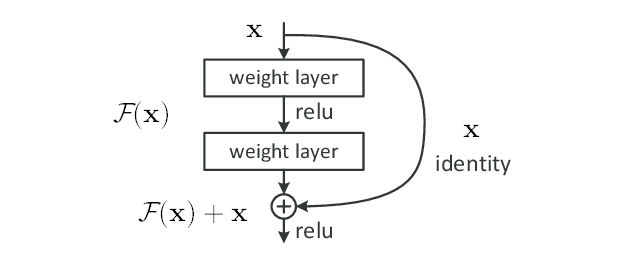
\includegraphics[width=8cm]{figures/resnet}
    \end{center}
    \caption{Structure of Residual Layer}
    \label{fig:Res-structure}
\end{figure}

\subsection{Batch Normalization}
\label{sec:BN}
Batch Normalization(BN) is a popular technique proposed by Ioffe and Szegedy \cite{ioffe2015batch} recently 
which alleviates a lot of headaches with properly initializing neural networks by forcing 
the activations throughout a network 
to take on a unit gaussian distribution at the beginning of the training according to \cite{cs231n}.
In deep learning, the latter layer could get inputs with a high variance and a mean value far from zero from the previous layer,
which is not good for stable training, to fix this problem, BN process every data with the equation:
$$y_{i}=\gamma \hat{x}_{i}+\beta \text { and } \hat{x}_{i}=\frac{x_{i}-\mu}{\sqrt{\sigma^{2}+\epsilon}}$$
Where $x_{i}$ is an activation for the $i^{th}$ example in the batch and $\hat{x}_{i}$ is the output after 
the process, $\mu$ and $\sigma^{2}$ are the mean value and variance of the activation over the batch, and
$\gamma$ and $\beta$ are trainable parameters.

In practice, we usually insert the BN layer between FC and non-linearities.
It has been shown that BN can make networks more robust to inappropriate
initialization. In addition, BN can be interpreted as doing preprocessing at every layer of a network, but 
integrated into the network itself in a differentiable manner, which is why BN is widely used nowadays.
For more details, please check the referenced paper \cite{ioffe2015batch}.

\section{Generative Adversarial Network}
Generative Adversarial Network(GAN) is one kind of deep learning approach originated from 
Goodfellow et al. \cite{goodfellow2014generative}. The idea of GAN is inspired from 
game theory: two neural networks contest against each other in a game(i.e. the training
process of deep learning), where one generator network tries to generate fake images while the 
other discriminator network tries to identify whether an image is real or fake. 
GAN models can learn
a loss that tries to classify if the output image is real or fake, while simultaneously training
a generative model to minimize this loss.
One advantage 
that GAN is more powerful than traditional CNN approach on image translation tasks is that 
GAN can produce clearer results for blurry images look obviously fake. Furthermore, we need 
expert knowledge and carefully designed loss function for traditional CNN models, while we 
only need to specify a high-level objective for GAN models: make the output looks like real, and then 
automatically learn a loss function for satisfying this goal, which is much more desirable.
\begin{figure}[H]
    \begin{center}
    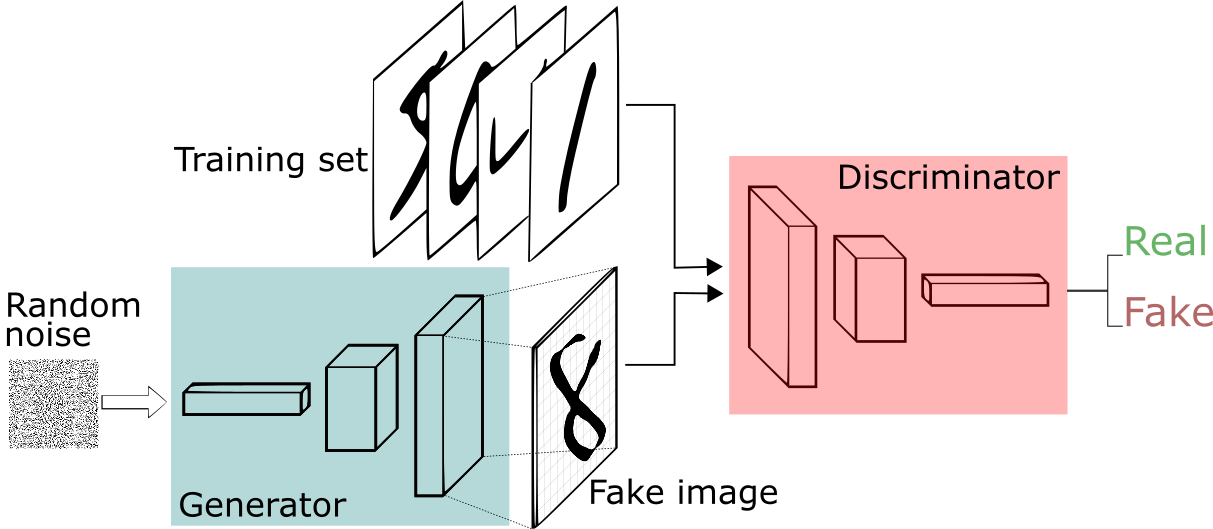
\includegraphics[width=8cm]{figures/GANs}
    \end{center}
    \caption{Structure of GANs}
    \label{fig:GANs-structure}
\end{figure}
\subsection{Conditional Generative Adversarial Network}
Conditional Generative Adversarial Network(cGAN) is a special kind of GAN whose input 
of the generator is not only the random noises, but also send in a condition image, the networks will learn 
to adapt and adjust their parameters to these additional condition inputs. For conventional GAN models, 
only the input noise can influence the output, however, for cGAN models, the conditional image can 
also influence the results. In image translation tasks, the encoded segmentation map is the condition 
we apply to the GAN model. Both pix2pix\cite{pix2pix2016} and pix2pixHD\cite{wang2018pix2pixHD} use 
this kind of GAN model.
\begin{figure}[H]
    \begin{center}
    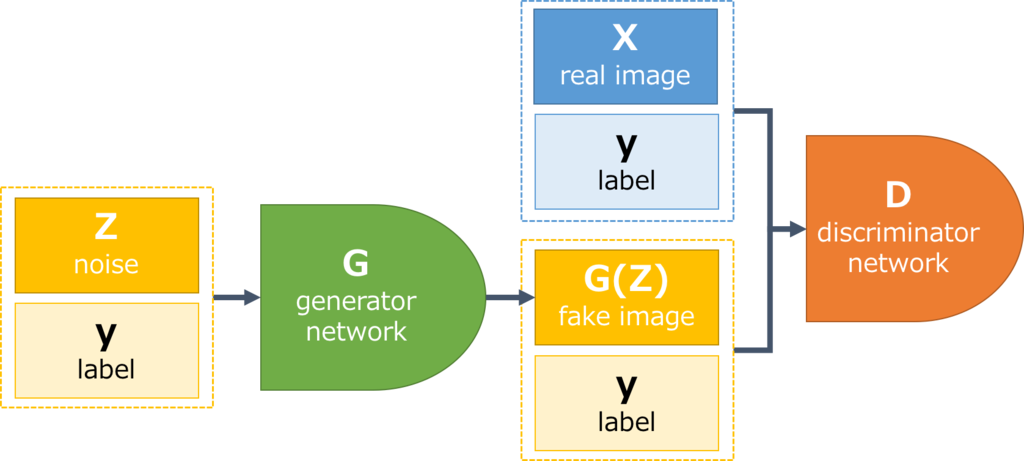
\includegraphics[width=8cm]{figures/cGANs}
    \end{center}
    \caption{Structure of conditional GANs}
    \label{fig:cGANs-structure}
\end{figure}

\section{Impact of COVID-19}
I decided to go back to Beijing after finishing my presentation of the 3rd year project on 16th March, 
my flight arrived at Xi'an, China at 23rd March, 
I had a low fever and was sent to a hospital for further checks, and fortunately, I am OK. 
After that, I was sent to a hotel and quarantine for 14 days in Xi'an, and then traveled back to Beijing and 
self-isolate for another 14 days at home according to the policies from the government. Generally speaking, I 
had quarantine for a month before I can work on my work wholeheartedly. Fortunately, I finished my demonstration 
before I left and the deadlines of the 3rd year project and other coursework have also been extended.

% Everything below here is commented material which is used by the
% emacs tex support system called auctex. If you're not an emacs user
% you can safely ignore it. If you do use emacs you should take a look
% at the local emacs or LaTeX WWW pages for more on emacs support for
% LaTeX.

% Local Variables:
% mode: latex
% TeX-master: "report"
% End:

